\documentclass[14pt,a4paper,oneside]{article}
\usepackage[14pt]{extsizes}
\usepackage[utf8]{inputenc}
\usepackage[russianb]{babel}
\usepackage{amsmath}
\usepackage{graphicx}
\usepackage{pdfpages}

\begin{document}
\begin{titlepage}
\centerline{Университет}\par
\centerline{Факультет}\par
\centerline{Кафедра}
\vfill
\centerline{\bf ФИО}\par
\bigskip
\centerline{\bf Название работы}\par
\bigskip
\centerline{Направление}\par
\centerline{Направленность}
\vfill
\centerline{\bf Научно-квалификационная работа}
\vfill
\begin{flushright}
{\bf Научный руководитель:}\\
к.ф.-м.н., доцент \\ ФИО
\end{flushright}
\vfill
\centerline{Москва~---~2019}
\end{titlepage}

\tableofcontents
\newpage
\section{Введение}
Важно заметить, что ни один из макропакетов для TeX’а не может расширить возможностей TeX {\it (всё, что можно сделать в LaTeX’е, можно сделать и в TeX’е без расширений)}, но, благодаря различным упрощениям, использование макропакетов зачастую позволяет избежать весьма изощрённого программирования.

Пакет позволяет автоматизировать многие \(S = a+b \) задачи набора текста и подготовки статей, включая набор текста на нескольких языках, нумерацию разделов и формул, перекрёстные ссылки, размещение иллюстраций и таблиц на странице, ведение библиографии и др. Кроме базового набора существует множество пакетов расширения LaTeX. Первая версия была выпущена {\bf Лесли Лэмпортом} в 1984 году; текущая версия, после создания в 1994 году испытывала некоторый период нестабильности, окончившийся к концу 1990-х годов, а в настоящее время стабилизировалась (хотя раз в год выходит новая версия).
График функции изображен на ~рис.\, \ref{fig:pic} на стр.\, \pageref{fig:pic}.
$$ S = a + b $$
$$ S = a \cdot b $$
$$ \frac{a}{b} $$
$$ a^{b+c}$$
$$ a_{b+c}$$
$$ \int e^{t} \, dt$$
$$ \int \limits_0^T e^{t} \, dt$$
$$ \delta \Phi $$ 
$$ d\Bigg(\frac{a}{b}\Bigg)$$
\begin{enumerate}
    \item Первый
    \item Второй
\end{enumerate}

\begin{figure}[t]
\centering
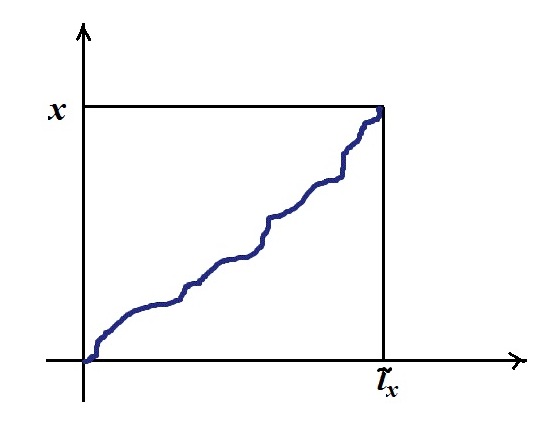
\includegraphics[scale=0.5]{1.jpg}
\caption{Описание картинки}
\label{fig:pic}
\end{figure}

\newpage
\section{Основная часть}
\subsection{Определение}
Важно заметить, что ни один из макропакетов для TeX’а не может расширить возможностей TeX (всё, что можно сделать в LaTeX’е, можно сделать и в TeX’е без расширений), но, благодаря различным упрощениям, использование макропакетов зачастую позволяет избежать весьма изощрённого программирования.
\subsection{Утверждение}
Пакет позволяет автоматизировать многие задачи набора текста и подготовки статей, включая набор текста на нескольких языках, нумерацию разделов и формул, перекрёстные ссылки, размещение иллюстраций и таблиц на странице, ведение библиографии и др. Кроме базового набора существует множество пакетов расширения LaTeX. Первая версия была выпущена Лесли Лэмпортом в 1984 году; текущая версия, после создания в 1994 году испытывала некоторый период нестабильности, окончившийся к концу 1990-х годов, а в настоящее время стабилизировалась (хотя раз в год выходит новая версия).

\includepdf[pages=-]{tab.pdf}
\newpage
\section{Заключение}
Важно заметить, что ни один из макропакетов для TeX’а не может расширить возможностей TeX (всё, что можно сделать в LaTeX’е, можно сделать и в TeX’е без расширений), но, благодаря различным упрощениям, использование макропакетов зачастую позволяет избежать весьма изощрённого программирования.

Пакет позволяет автоматизировать многие задачи набора текста и подготовки статей, включая набор текста на нескольких языках, нумерацию разделов и формул, перекрёстные ссылки, размещение иллюстраций и таблиц на странице, ведение библиографии и др. Кроме базового набора существует множество пакетов расширения LaTeX. Первая версия была выпущена Лесли Лэмпортом в 1984 году; текущая версия, после создания в 1994 году испытывала некоторый период нестабильности, окончившийся к концу 1990-х годов, а в настоящее время стабилизировалась (хотя раз в год выходит новая версия).
\newpage

\end{document}
